\chapter{Little's Theorem}	% *NOT* \OnePageChapter
Little's Theorem states:
\begin{equation}
    N = \lambda T
\end{equation}
Where N is the average number of packets in a queue, T is the average time a packet spends queuing and $\lambda$ is the average rate of arrivals to the queue.
\par Let us first make some definitions:
\begin{itemize}
    \item N($\tau$) is the number of packets in the system at time $\tau$.
    \item $\alpha(\tau)$ is the number of packets which arrived in the interval [0; $\tau$].
    \item $\beta(\tau)$ is the number of packets departed in the interval [0;$\tau$].
    \item t\textsubscript{i} is the time at which the i\textsuperscript{th} packet arrived.
    \item T(i) is the time spent queuing by the i\textsuperscript{th} packet.
\end{itemize}
If N\textsubscript{t} is the mean value of N($\tau$) taken over the interval [0;t] then it is clear that:
\begin{equation}
    N\textsubscript{t} = \frac{1}{t}\int_{0}^{t} N(\tau) d\tau
\end{equation}
We next define the average arrival rate over the time period [0;t].
\begin{equation}
    \lambda\textsubscript{t} = \frac{\alpha(t)}{t}
\end{equation}
and,again,we assume that the following limit exists:
\begin{equation}
    \lambda = \lim_{t\to\infty} \lambda(t)
\end{equation}
Finally, the average delay experienced by packets who enter the system at times in [0;t]is given by:
\begin{equation}
    T\textsubscript{t} = \sum_{i=1}^{\alpha(t)} \frac{T(i)}{\alpha(t)} 
\end{equation}
\begin{figure}[h!]
    \centering
    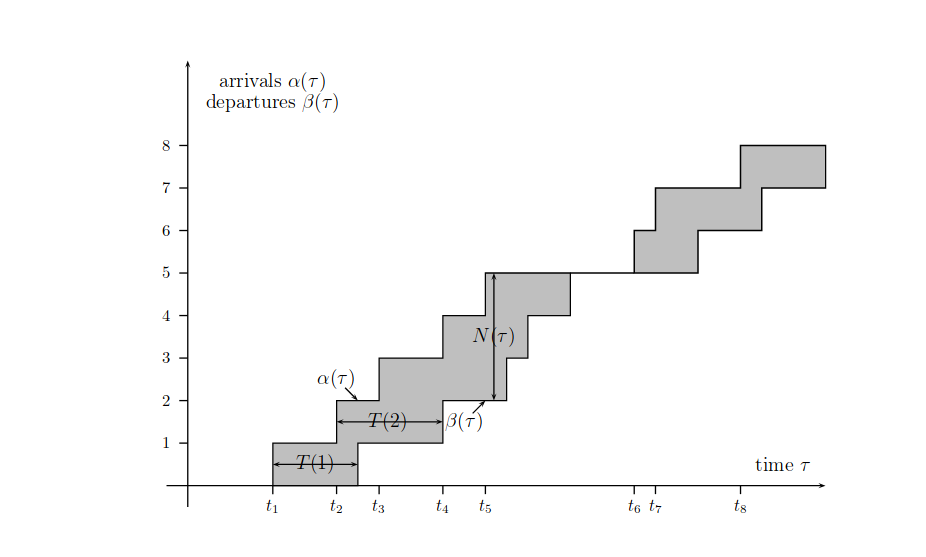
\includegraphics[scale=0.5]{Thesis/figs/appendix.png}
    \caption{Little's Theorem in a FIFO system}
    \label{fig:my_label}
\end{figure}
\par From fig A.1, we note that at any time $\tau$:
\begin{equation}
    N(\tau) = \alpha(\tau) - \beta(\tau)
\end{equation}
It is clear that if we choose a time t when the system again be comes empty then we can calculate the area of the shaded area A(t):
\begin{equation}
    A(t) = \int_{0}^{t} N(\tau) d\tau
\end{equation}
However,equally, we can consider the shaded area to be composed of horizontal strips of height 1 and width T(i) (for the i\textsuperscript{th} packet).In this case,we have:
\begin{equation}
    A(t) = \sum_{i=1}^{\alpha(t)}T(i)
\end{equation}
Setting these equations equal and dividing each side by t gives us:
\begin{equation}
    N\textsubscript{t} = \lambda\textsubscript{t} T\textsubscript{t}
\end{equation}
which, if we take the limit as (t-> $\infty$) becomes Little's Theorem as required.